\documentclass{article}
\usepackage[utf8]{inputenc}
\usepackage{graphicx}
\usepackage{amsmath}
\usepackage{amsfonts}
\usepackage{amsbsy}
\usepackage{mathrsfs}
\usepackage{appendix}
\usepackage{amsthm}
\usepackage{bbold}
\usepackage{epstopdf}
\usepackage{stmaryrd}
\usepackage[]{algorithm2e}
\usepackage{hyperref}

\title{Reading report for continuous attractor network}
\author{Leman FENG\\ Email: flm8620@gmail.com\\Website: lemanfeng.com}

\begin{document}
	\maketitle
	\section{Background}
	This paper \cite{romani2010continuous} goes directly to the study of a specific case of continuous attractor network without much introduction to basic concepts. So I read other materials about continuous attractor networks before going through the paper.
	
	\subsection{Hopfield network}
	We have seen Hopfield network in the course. In one Hopfield network, many neural units $\{x_i\}_i$ exists. Each unit can only take binary values. The connection strength between each pair of units $w_{ij}$ is symmetrical.
	
	The update rule is simply:
	\begin{equation}
	x_i \leftarrow
	\begin{cases}
	+1 & \text{if} \sum_{j}w_{ij}x_j \geq \theta_i\\
	-1 & \text{otherwise}
	\end{cases}
	\end{equation}
	
	\subsection{Attractor network}
	Attractor network is a general concept. We will often see definition like: An attractor network consists of $N$ neural units connected such that the global dynamics becomes stable in a $D$ dimensional space and $N>>D$.
	
	This implies that attractor network deal with continuous values and continuous update rules. Or more direct, real-valued nodes and differential equations for update rules. So all possible states of network is $\mathbb{R}^N$. And all stable states form a lower dimensional manifold in $\mathbb{R}^N$. Stable states are called attractors. According to the shape of the manifold, there are points, line, ring, plane attractors and so on.
	
	So from my point of view, the attractor network is just the dynamics of a set of real-valued variables ruled by a set of differential equations. It's more like a pure mathematical objects which can be applied in many domains, such as physics, the study of pendulum's dynamics. And biological interpretation is just another possibility.
	
	For biological interpretation, one natural way to construct an attractor network is to extend the Hopfield network in a continuous version. So for each node the update rule is
	\begin{equation}
	\frac{\mathrm{d}x_i}{\mathrm{d}t} = -\lambda x_i + f(\sum_j w_{ij} x_j)
	\end{equation}
	where $f$ is the transfer function.
	
	From this update rule, we can see that without connection from other units, the activity of one neural unit will decay exponentially to zero.
	
	\subsection{Continuous attractor network}
	Then we finally reach the continuous attractor network. The first we need thing to understand is what does it mean by "continuous". Because attractor network deals already with continuous values and differential equations.
	
	From the name, it seems that it talks about a continuous set of attractor. But we already have the line, ring and plane attractors in a normal attractor network. So this must not be the meaning of "continuous". The formal definition of a continuous attractor is very abstract, including minimal closed set of attractors which satisfy certain properties, according to \cite{CANN}. While I didn't find any formal definition for Continuous attractor network, it seems that the only way to have a continuous attractor is to have infinite neural units in network \cite{trappenberg2003continuous}. And the infinite neural units form a continuum of neurons. This continuum of neurons doesn't come from the definition, but from the result of the definition of continuous attractor network.
	
	Since we talks about infinite neural units, it makes no sense to talk about one neural unit. We can only define neural units as a density function $\nu(x)$ over a manifold $\mathbf{X}$. It's just like the difference between discrete and continuous probability distribution. And the weights between neurons is no longer a matrix, but a function defined on the Cartesian product of $\mathbf{X}$ : $W:\mathbf{X}\times \mathbf{X} \rightarrow \mathbb{R} $. 
	
	We use $\mathbf{m}:\mathbf{X}\rightarrow\mathbb{R}$ to denote the activity of network. Then the update rule becomes:
	\begin{equation}
	\frac{\mathrm{d}\mathbf{m}(x)}{\mathrm{d}t} = -\lambda \mathbf{m}(x) + f(\int_{\mathbf{X}}\nu(x)W(x,y)m(y)\mathrm{d}y)
	\end{equation}
	
	\section{Network structure}
	After the study of basic concepts, I dig into this paper \cite{romani2010continuous}. The introduction section is very abstract and I can hardly understand author's motivation about the superposition of multiple maps. So I decide to study the first example with two maps.
	
	The author use the word "map" to refer a single manifold. He defines two circular one-dimensional maps $\Theta_A,\Theta_B$ and the coordinates system are $\theta_A\in[0,2\pi),\theta_B\in[0,2\pi)$. And the neurons live on the Cartesian product of these two maps. And neurons are identified by pair of labels $(\theta_A,\theta_B)$, with their density distribution $\nu(\theta_A,\theta_B)$. The neurons actually live on a surface of torus, circular in both directions.
	
	Despite it makes no sense to say one neuron at coordinate $(\theta_A,\theta_B)$, I will still use this way to express one infinitesimal neighborhood of neuron continuum located near $(\theta_A,\theta_B)$, just as the author does.
	
	The weight between two neurons $(\theta_A,\theta_B)$ and $(\theta_A',\theta_B')$ is given by 
	\begin{equation}
	W((\theta_A,\theta_B),(\theta_A',\theta_B')) = \frac{J_1}{2}[\cos(\theta_A-\theta_A')+\cos(\theta_B-\theta_B')+J_0]
	\end{equation}
	although the author defines $W$ using the expression $W(\theta_A-\theta_A',\theta_B-\theta_B')$, which confused me a lot at the beginning, I still want to write the right definition of weight function to clarify that each neuron is identified by two coordinates, not one.
	
	From this definition, we can see that for neurons close to each other, they have positive interaction between them. For neurons far away from each other, they will have less interaction or even negative interaction, or inhibition, to each other.
	
	And the dynamics is given by 
	\begin{equation}
	\begin{split}
	\tau &\dot{\mathbf{m}}(\theta_A,\theta_B) = -\mathbf{m}(\theta_A,\theta_B) +\\ &\max[0,\int_{\Theta_A\times\Theta_B}\nu(\theta_A',\theta_B')W((\theta_A,\theta_B),(\theta_A',\theta_B'))\mathbf{m}(\theta_A',\theta_B')\mathrm{d}\theta_A'\mathrm{d}\theta_B' + I]
	\end{split}
	\end{equation}
	$I$ indicates the uniform external current.
	
	Until now, we didn't define the density of neurons $\nu(\theta_A,\theta_B)$. The author used a simple way to build a correlated/uncorrelated distribution. By correlation, the author means that we can think about $\nu(\theta_A,\theta_B)$ as a probability distribution (up to a constant), then consider the correlation of two random variable $\nu(\theta_A),\nu(\theta_B)$ which follows the marginal distribution of $\nu(\theta_A,\theta_B)$.
	
	The author used a change of variables. Let's redefine $\theta_A=(\theta-\mu r), \theta_B=(\theta+\mu r)$, modulo $2\pi$, for $(\theta,r)$ uniformly distributed on $\Theta\times R = [0,2\pi)\times[-\pi/2,\pi/2]$, and a parameter $\mu\in[0,1]$.
	
	For me, this definition can be summarized as : let's create uniform neuron continuum over $\Theta_A\times\Theta_B=[0,2\pi)\times[0,2\pi)$, then delete those neurons whose two coordinates are too far apart : the distance between $\theta_A$ and $\theta_B$ over a circular ring is larger than $\mu\pi$.
	
	After this deletion, although the two maps are correlated (if $\mu<1$), the marginal distribution is still uniform over respectively $\Theta_A$ and $\Theta_B$, simply because of the periodic maps and the symmetrical deletion.
	
	\section{Dynamics}
	The author studied the type of attractors in this network. It's hard to study directly the dynamics of the whole network. So the author used the first three Fourier components of network activity : $Z_A,Z_B,\eta$, which is a natural way of simplification because both maps are periodic:
	\begin{equation}
	\begin{split}
	Z_A &= \int_{\Theta_A\times\Theta_B} e^{i\theta_A} \mathbf{m}(\theta_A,\theta_B) v(\theta_A,\theta_B)=\rho_A e^{i\Psi_A}\\
	Z_B &= \int_{\Theta_A\times\Theta_B} e^{i\theta_B} \mathbf{m}(\theta_A,\theta_B) v(\theta_A,\theta_B)=\rho_B e^{i\Psi_B}\\
	\eta &= \int_{\Theta_A\times\Theta_B} \mathbf{m}(\theta_A,\theta_B) v(\theta_A,\theta_B)\\
	\end{split}
	\end{equation}
	$Z_A, Z_B$ are respectively the first Fourier components of marginal activity on $\Theta_A$ and $\Theta_B$, and $\eta$ is just the mean value.
	
	By using again the dynamics of network, we can get the dynamics of these three variables. Notice that $Z_A, Z_B$ are complex numbers, whose modulus $\rho_A,\rho_B$ indicate the strength of peaks in marginal activity, and whose angles $\Psi_A,\Psi_B$ indicate the position of peaks in marginal activity. So in total five degrees of freedom. The author again used a change of variables to introduce dimensionless parameters in function of these five degrees of freedom. The final reduced dynamics are represented by five parameters: $(\gamma, \alpha, \sigma, \Psi_+, \Psi_-)$, with their definitions:
	\begin{equation}
	\begin{split}
	\gamma&=\frac{\rho_B-\rho_A}{\rho_B+\rho_A},\quad \alpha=\frac{J_1}{I}\frac{\rho_B+\rho_A}{2}\\
	\sigma&=\frac{I+J_0\eta}{\alpha I},\quad\\
	\Psi_+ &= \frac{\Psi_A+\Psi_B}{2},\quad \Psi_- = \frac{\Psi_A-\Psi_B}{2}
	\end{split}
	\end{equation}
	The meaning of each parameter is:
	\begin{itemize}
		\item $\gamma\in[-1,1]$, difference of bump magnitude in two maps $\Theta_A,\Theta_B$
		\item $\alpha>0$, scaling factor of the whole activity
		\item $\sigma\in[-1,1]$, spatial size of bump, -1 means no activity and 1 means all neurons are equally active. 
		\item $\Psi_+$, the location of bump in $\Theta$, or the averaged location in $\Theta_A$ and $\Theta_B$, which isn't important because network is periodic on $\Theta$. This parameter is ignore during the study of attractor.
		\item $\Psi_-$, the location of bump in $R$, or the difference of location in $\Theta_A$ and $\Theta_B$. This parameter can only be ignore when $\mu=1$, where the network degenerate to a torus.
	\end{itemize}
	
	\section{Attractors}
	The authors shown that, depend on the value of $J_1$ and $\mu$, there are four kinds of attractors: Homogeneous, Single ring, Double ring and Cylinder. The first Homogeneous case is not interesting. The three latter cases comes from the distinction on value pair $(\gamma,\Psi_-)$. The relation is shown in the table:
	\begin{center}
		\begin{tabular}{ | c | c | c | }
			\hline
			               & $\gamma=0$  & $\gamma\neq 0$ \\ \hline
			$\Psi_-=0$     & Single ring & Double ring \\ \hline
			$\Psi_-\neq 0$ & Cylinder    & Impossible  \\
			\hline
		\end{tabular}
	\end{center}
	\subsection{Simulation}
	To reproduce the result of the three types of attractor, I implemented in Matlab a numerical simulation of the network. The code is available online at \href{https://github.com/flm8620/Continuous-attractor-network}{my github}.I take a discretization of $M\times N$ on the space of $\Theta\times R = [0,2\pi)\times[-\pi/2,\pi/2]$. For each type of attractors I pick one and show them in Fig \ref{fig:type}.
	
	\begin{figure}[h]
		\centering
		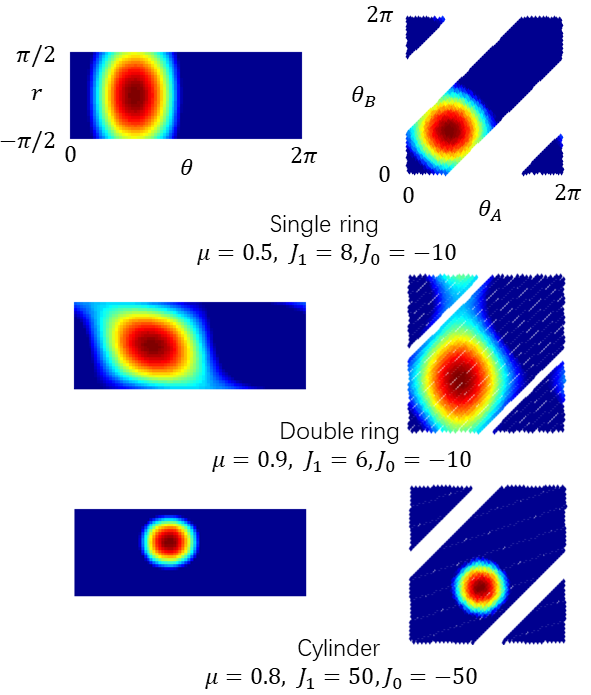
\includegraphics[width=12cm]{figures.png}
		\caption{Three types of attractor. Each row shows one attractor in two different coordinates, $\Theta\times R$ and $\Theta_A\times\Theta_B$}
		\label{fig:type}
	\end{figure}

	\section{Turning curves}
	The author then tried a non-uniform external input $I$ to see the behavior of network. The input chosen by author is 
	\begin{equation}
	I'(t) := I + \varepsilon I_E(\theta_A-\Psi(t)),\quad I_E(x) := cos(x)
	\end{equation}
	which is a bump signal in the map $\Theta_A$. 
	
	This signal let the network have a bump in its activity according to the position of signal $\Psi(t)$. 
	
	If the signal $\Psi(t)=\Psi$ is constant over time, and if the parameter of network belongs to Single ring or Double ring, then the position of bump in network's activity will be the same in both $\Theta_A$ and $\Theta_B$, equal to $\Psi$. While if the network belongs to Cylinder type, we can only say the average of bump in $\Theta_A$ and $\Theta_B$ equals to $\Psi$.
	
	What's interesting is when the signal $\Psi(t)=vt$ rotates in $\Theta_A$, for the network of type Cylinder, the position of bump will depend not only on the current position of signal $\Psi(t)$, but also the direction of rotation ($v>0$ or $v<0$). As shown in Fig \ref{fig:moving}, the Cylinder attractor will follow the external signal until it hits the wall (absence of neurons), and continue gliding along the wall. And author interpret this as some kind of memory ability of the network.
	
	\begin{figure}[h]
		\centering
		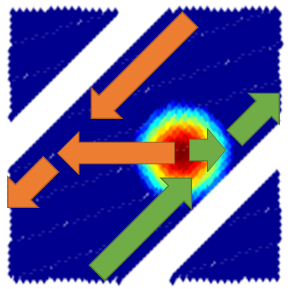
\includegraphics[width=12cm]{moving.png}
		\caption{Path of bump in activity when input a rotating signal in $\Theta_A$ (horizontal axis). Only Cylinder attractor will behave differently according to the direction of rotation. (Path in orange and green)}
		\label{fig:moving}
	\end{figure}

	\section{Morph sequence}
	The first part of paper discuss only about the case of two maps. Then author talks about morph sequence, which is a limit of infinite maps. Before understanding morph sequence, I felt confused of the relation between neurons and maps until I figured out these two equivalent descriptions. I think it's better to clarify these two description from my point of view to ease the comprehension.
	
	The first description is to think that the existence of neurons is independent from maps. Or more precisely, for a continuous attractor network, neurons live in a space that occupy a set of unit measure. Then we put these neurons in different maps. Each neuron has its appearances in all maps. And in each map, all neurons occupy different location with a density like a probability distribution whose measure is also one. So for each neuron, we can track its appearances in all maps. And for the connection strength between two neurons, the author makes it equals to the averaged connection strength in all maps between locations occupied by two neurons. Just as shown in Fig \ref{fig:morph} and Fig \ref{fig:morph_more}.
	\begin{figure}[h]
	\centering
	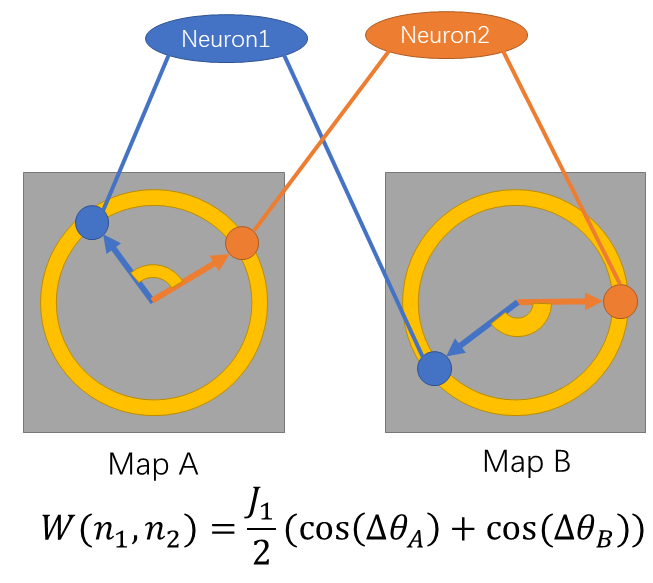
\includegraphics[width=8cm]{morph.png}
	\caption{Each neuron appears in both maps. Weight between neurons is the sum of weight in all maps}
	\label{fig:morph}
	\end{figure}

	\begin{figure}[h]
		\centering
		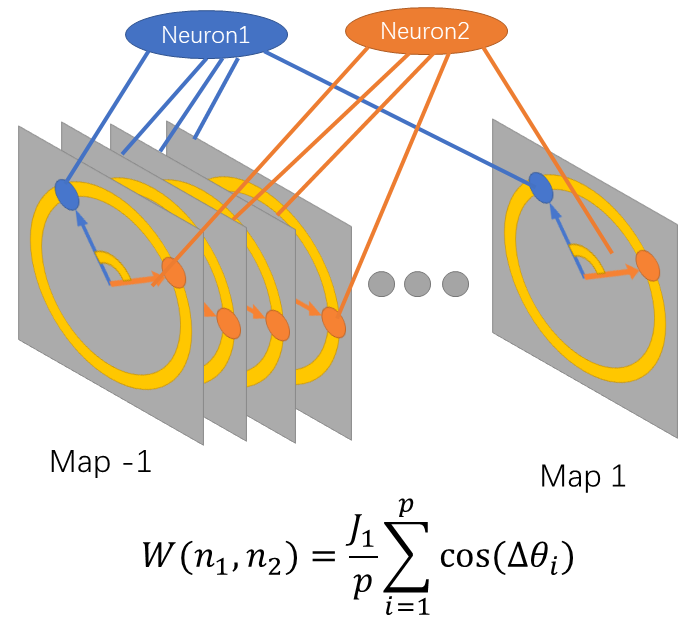
\includegraphics[width=8cm]{morph_more.png}
		\caption{Each neuron appears in all maps. Weight between neurons is the sum of weight in all maps.}
		\label{fig:morph_more}
	\end{figure}
	
	
	The second description is to put neurons directly in the space formed by the Cartesian product of all maps. The density of neurons is described by a probability distribution over this space. Each neuron only appears one time at one location in this space. And there isn't any independent existence of neuron without this space. The connection strength between two neurons is defined by one function that takes two location in this space as variables.
	
	Someone may find it redundant to use two equivalent descriptions. But I think it's useful to switch between these two descriptions when needed. When the author introduce infinite morph sequence of maps, it's easier to use the first description by imagining adding a new map at a time. While the second method is suitable for mathematical formula, for example, the correlation between maps is actually the correlation between two marginal variables following only one probability distribution in only one probability space instead of a series of them.
	
	I'm still not fully understand the motivation of studying the morph sequence. I guess one idea is that, animal brain has a fixed structure of neurons and they can handle different task in different environment. Using the first description, the existence of neurons is independent. And they can store different maps (or connection modes). In each environment the brain will activate the correspondent map. And external signals given in this environment applied also on the very map, but there will be other activities in other maps, as shown by previous result.
\bibliographystyle{unsrt}
\bibliography{sample}
\end{document}
